% Chapter Template

\chapter{Theoretical Background} % Main chapter title

\label{Chapter2} % Change X to a consecutive number; for referencing this chapter elsewhere, use \ref{ChapterX}

\lhead{Chapter 2. \emph{Theoretical Background}}
This chapter is devoted to present the theoretical foundations and formalism of Density Functional Theory (DFT) and related methods required for the development of the results presented in this work. Starting with the many-body Schrödinger equation, this chapter covers the Born-Oppenheimer approximation, the Hartree-Fock approximation, Hohenberg-Kohn theorems, the Kohn-Sham equations, exchange-correlation functionals, and definitions on Ab initio molecular dynamics (AIMD) and machine learning force fields (MLFFs), along with implementation details in the Vienna Ab initio Simulation Package (VASP).

Ultimately, this chapter aims to provide a comprehensive understanding of the theoretical framework that underpins the computational methods utilised in this work, enabling the reader to grasp the principles and assumptions that govern the simulations and analyses performed throughout.

\section{Many Body Schrödinger Equation}
In the realm of materials science, comprehending particle behaviour within a system inevitably demands resorting to intricate principles of quantum mechanics. Our journey shall commence by describing the physical laws that shape the interactions among particles constituting a system---electrons and nuclei alike. 

\subsection{The Coulomb Interaction}

Materials may be thought of as complex assemblies of electrons and nuclei, held together by a delicate balance between attractive Coulomb interactions---primarily between electrons and nuclei---and repulsive interactions between like-charged particles, such as electron-electron and nucleus-nucleus pairs, which govern the overall dynamics of the material system\supercite{giustino2014materials, sholl2023density, kaxiras2003atomic}.  From classical electrostatics, these interactions can be mathematically expressed as follows: 

\begin{itemize}
\item Electron-electron interactions 
  \begin{equation}
    \label{eq1}
    \hat{V}_{ee} = \frac{1}{2} \sum_{i\neq j} \frac{e^2}{4\pi\epsilon_0 |\mathbf{r}_i - \mathbf{r}_j|}
  \end{equation}
\item Electron-nucleus interactions 
  \begin{equation}
    \label{eq2}
    \hat{V}_{nn} = \frac{1}{2} \sum_{I\neq J} \frac{e^2}{4\pi\epsilon_0} \frac{Z_I Z_J}{|\mathbf{R}_I - \mathbf{R}_J|}
  \end{equation}
\item Electron-nuclei interactions 
\begin{equation}
    \label{eq3}
    \hat{V}_{en} = -\sum_{i\neq I} \frac{e^2}{4\pi\epsilon_0} \frac{Z_I}{|\mathbf{r}_i - \mathbf{R}_I|}
  \end{equation}
\end{itemize}

where $e$ is the electronic charge, $\epsilon_0$ is the vacuum permittivity, $Z_I$ and $Z_J$ are the atomic numbers of nuclei $I$ and $J$, respectively, and $\mathbf{r}_i$ and $\mathbf{R}_I$ are the position vectors of electrons and nuclei, respectively. Moreover, we must also consider the kinetic energy of the collection of electrons and nuclei
\begin{equation}
    \label{eq4}
    \hat{T} = -\sum_i \frac{\hbar^2}{2m_e} \nabla_i^2 - \sum_I \frac{\hbar^2}{2M_I} \nabla_I^2
\end{equation}
where $\hbar$ is the reduced Planck's constant, $m_e$ is the electron mass, and $M_I$ is the mass of the nucleus $I$.

\subsection{The Time-Independent Schrödinger Equation}
The Time-Independent Schrödinger Equation (TISE) lies at the heart of non-relativistic quantum mechanics, providing a mathematical framework to describe stationary electronic states of quantum systems. It takes the following form:
\begin{equation}
  \label{eq5}
  \hat{H} \psi(\mathbf{r}) = E \psi(\mathbf{r})
\end{equation}
where $\hat{H}$ is the Hamiltonian of the system, encompassing both kinetic and potential energies, $\psi(\mathbf{r})$ is the wavefunction of the system, and $E$ is the energy eigenvalue associated with the state described by $\psi(\mathbf{r})$.  It is important to note that Equation \ref{eq5} is only applicable to a single particle, yet a material system is composed of many electrons (N) and nuclei (M) with spatial coordinates $\mathbf{r}_1, \mathbf{r}_2, \ldots, \mathbf{r}_N$ and $\mathbf{R}_1, \mathbf{R}_2, \ldots, \mathbf{R}_M$, respectively. Therefore, we must introduce a so-called many-body wavefunction given by:
\begin{equation}
  \Psi(\mathbf{r}_1, \mathbf{r}_2, \ldots, \mathbf{r}_N, \mathbf{R}_1, \mathbf{R}_2, \ldots, \mathbf{R}_M)
  \label{eq5b}
\end{equation}
On this basis, the many-body version of Equation \ref{eq5} shall be constructed by combining the kinetic (Equation \ref{eq4}) and potential (Equations \ref{eq1}, \ref{eq2}, and \ref{eq3}) energy contributions, leading to the following expression:
\begin{equation}
  \label{eq6}
  \begin{split}
    \left[
      -\sum_i \frac{\hbar^2}{2m_e} \nabla_i^2 
      - \sum_I \frac{\hbar^2}{2M_I} \nabla_I^2 
      + \frac{1}{2} \sum_{i\neq j} \frac{e^2}{4\pi\epsilon_0 |\mathbf{r}_i - \mathbf{r}_j|} +\right. \\
      \left. \frac{1}{2} \sum_{I\neq J} \frac{e^2}{4\pi\epsilon_0} \frac{Z_I Z_J}{|\mathbf{R}_I - \mathbf{R}_J|} 
      - \sum_{i, I} \frac{e^2}{4\pi\epsilon_0} \frac{Z_I}{|\mathbf{r}_i - \mathbf{R}_I|}
    \right]\Psi = E_{\text{tot}} \Psi
  \end{split}
\end{equation}
Equation \ref{eq6} provides a complete description of the stationary states of a non-relativistic many-body system, under time-independent conditions and in the absence of external fields. Additionally, we can achieve a more compact formulation by introducing the concept of atomic units. To this end, let us consider the simplest electron-nucleus system---the hydrogen atom---where the electron orbital has an average radius $a_0 \approx 0.529 \, \text{Å}$. Thereby, the Coulomb energy for such a system is given by:
\begin{equation}
  \label{eq7}
  E_{\text{Ha}} = \frac{e^2}{4 \pi \epsilon_0 a_0}
\end{equation}
where 'Ha' stands for Hartree. Within this framework, the Hartree energy represents the Coulomb interaction between two fundamental charges separated by a distance of one Bohr radius ($a_0$). Moreover, the angular momentum quantisation condition for the electron in the hydrogen atom is given by
\begin{equation}
  \label{eq8}
  m_e v a_0 = \hbar
\end{equation}
Additionally, the equilibrium condition between the nuclear attraction and the electron's centrifugal force can be expressed as:
\begin{equation}
  \label{eq9}
  \frac{e^2}{4 \pi \epsilon_0 a_0^2} = \frac{m_e v^2}{a_0}
\end{equation}
By combining Equations \ref{eq7}, \ref{eq8}, and \ref{eq9}, we derive the 
following relationships:
\begin{equation}
  \label{eq10}
  \frac{e^2}{4 \pi \epsilon_0 a_0} = \frac{\hbar^2}{m_e a_0^2}
\end{equation}
\begin{equation}
  \label{eq11}
  \frac{1}{2} m_e v^2 = \frac{1}{2}E_{\text{Ha}}
\end{equation}
This latter relation showcases that the kinetic energy is of the same order as $E_\text{Ha}$, rendering it convenient to normalise Equation \ref{eq6} by this quantity:
\begin{equation}
  \label{eq12}
  \begin{split}
    \left[
      -\sum_i \frac{1}{2}a_0^2 \nabla_i^2 
      - \sum_I \frac{1}{2} \frac{1}{(M_I/m_e)} \nabla_I^2 
      + \frac{1}{2} \sum_{i\neq j} \frac{a_0}{|\mathbf{r}_i - \mathbf{r}_j|}\right. \\
      \left. +  \frac{1}{2} \sum_{I\neq J} Z_I Z_J \frac{a_0}{|\mathbf{R}_I - \mathbf{R}_J|} 
      - \sum_{i, I} Z_I \frac{a_0}{|\mathbf{r}_i - \mathbf{R}_I|}
    \right]\Psi = \frac{E_{\text{tot}}}{E_{\text{Ha}}} \Psi
  \end{split}
\end{equation}
A final simplification involves setting our energy units to Ha, distance units to $a_0$, and mass units to $m_e$. The last missing constant $e$ is set to 1, leading to the following expression: 
\begin{equation}
  \label{eq13}
  \begin{split}
    \left[
      -\sum_i \frac{\nabla_i^2}{2}
      - \sum_I \frac{\nabla_I^2}{2 M_I} 
      + \frac{1}{2} \sum_{i\neq j} \frac{1}{|\mathbf{r}_i - \mathbf{r}_j|} + \right. \\
      \left. \frac{1}{2} \sum_{I\neq J} \frac{Z_I Z_J} {|\mathbf{R}_I - \mathbf{R}_J|} 
      - \sum_{i, I} \frac{Z_I}{|\mathbf{r}_i - \mathbf{R}_I|}
    \right]\Psi = E_{\text{tot}} \Psi
  \end{split}
\end{equation}

Ultimately, even though Equation \ref{eq13} provides an exact method capable of yielding various properties of a material system---such as elastic, thermal, and electronic properties---a combination of mathematical complexity and computational limitations renders it intractable to solve for any realistic system. Moreover, the wavefunction contains vastly more information than is necessary to describe most observable properties of a material. Therefore, we must resort to alternative formulations that allow us to extract only the relevant information from the wavefunction whilst reducing the computational cost of the calculations. The remainder of this chapter is dedicated to presenting such alternative approaches that ultimately lead to the computational methods employed throughout this work.

%-----------------------------------
%	SUBSECTION 1
%-----------------------------------
\section{The Born-Oppenheimer Approximation}
For atoms in a solid, we can think of nuclei as being held immobile in a fixed position, while electrons instantaneously react to any nucleus's movement. This assumption is based on the fact that nuclei are much heavier than electrons---by three to four orders of magnitude---making the former behave like classical particles. Thereby, we can rewrite the many-body wavefunction as a product of two wavefunctions:
\begin{equation}
  \Psi(\mathbf{r}_1, \mathbf{r}_2, \ldots, \mathbf{r}_N, \mathbf{R}_1, \mathbf{R}_2, \ldots, \mathbf{R}_M) = \psi_{\mathbf{R}}(\mathbf{r}_1, \mathbf{r}_2, \ldots, \mathbf{r}_N)\chi(\mathbf{R})
  \label{eq14}
\end{equation}
where $\psi_{\mathbf{R}}$ is the electronic wavefunction parametrised by the nuclear positions $\mathbf{R}$, and $\chi$ is the nuclear wavefunction. Furthermore, this significant mass disparity enables a systematic approximation scheme, in which the electronic wavefunction is solved for fixed nuclei, and its solution is used as an effective potential for the nuclear dynamics afterwards. First, nuclei' kinetic energy is neglected, as their positions are assumed to be fixed: 
\begin{equation}
  \label{eq15}
  \sum_I \frac{\nabla_I^2}{2 M_I} = 0
  \quad \text{and} \quad  E = E_{\text{tot}} - \sum_{I<J} \frac{Z_I Z_J}{|\mathbf{R}_I - \mathbf{R}_J|}
\end{equation}
Following, we define the Coulomb potential of the nuclei experienced by the electrons as:
\begin{equation}
  \label{eq16}
  V_{\text{n}}(\mathbf{r}) = - \sum_{I} \frac{Z_I}{|\mathbf{r} - \mathbf{R}_I|}
\end{equation}
Then, Equation \ref{eq13} can be rewritten as:
\begin{equation}
  \label{eq17}
  \left[
    -\sum_i \frac{\nabla_i^2}{2} + \sum_i V_{\text{n}}(\mathbf{r}_i) + \frac{1}{2} \sum_{i\neq j} \frac{1}{|\mathbf{r}_i - \mathbf{r}_j|} 
  \right] \Psi = E \Psi 
\end{equation}
Finally, by using Equation \ref{eq14}, we can define the electronic and nuclear Schrödinger equations as follows:
\begin{equation}
  \label{eq18}
  \left[
    -\sum_i \frac{\nabla_i^2}{2} + \sum_i V_{\text{n}}(\mathbf{r}_i) + \frac{1}{2} \sum_{i\neq j} \frac{1}{|\mathbf{r}_i - \mathbf{r}_j|} 
  \right] \psi_{\mathbf{R}} = E_{\mathbf{R}} \psi_{\mathbf{R}}
\end{equation}
\begin{equation}
  \label{eq19}
  \left[
    -\sum_I \frac{\nabla_I^2}{2 M_I} + \sum_{I<J} \frac{Z_I Z_J}{|\mathbf{R}_I - \mathbf{R}_J|} + E(\mathbf{R}_1,\dots,\mathbf{R}_M)\right] \chi(\mathbf{R}) = E_{\text{tot}} \chi(\mathbf{R})
\end{equation}
where $E_{\mathbf{R}}= E(\mathbf{R}_1,\dots,\mathbf{R}_M)$ is the electronic surface energy, which is a function of the nuclear positions, and serves as an effective potential shaping the nuclear dynamics. 

%-----------------------------------
%	SUBSECTION 2
%-----------------------------------

\section{Hartree-Fock Approximation}
The essence of the Hartree-Fock approximation (HFA) is to approximate the interacting many-electron system (Equation \ref{eq17}) by a set of non-interacting single-particle problems subject to an effective mean-field potential\supercite{martin2016interacting, helgaker2014molecular, feng2005introduction}. As a means to this, we first rewrite the total wavefunction for a system with N electrons as the product of single-electron wavefunctions---often referred to as the Hartree approximation\supercite{Hartree1928}---as showcased in Equation \ref{eq20}. 
\begin{equation}
  \Psi^H(\mathbf{r}_1, \dots, \mathbf{r}_N) = \prod_{i=1}^N \phi_i(\mathbf{r}_i)
  \label{eq20}
\end{equation}
Following, we construct the total energy functional as the expectation value of the Hamiltonian operator:
\begin{equation}
  \label{eq21}
\begin{aligned}
  E^{H}[\{\phi_i\}] &= \bigg\langle \Psi^H \bigg| \hat{H} \bigg| \Psi^H \bigg\rangle 
\end{aligned}
\end{equation}
Expanding Equation \ref{eq21}:
\begin{equation}
  \label{eq22}
  \begin{split}
    E^{H}[\{\phi_i\}] &= \sum^N_{i=1} \int \phi_i^*(\mathbf{r}) \left(-\frac{\nabla^2}{2} + V_{\text{n}}(\mathbf{r})\right) \phi_i(\mathbf{r}) d\mathbf{r}  + \frac{1}{2} \sum_{i\neq j} \int\int \frac{|\phi_i(\mathbf{r})|^2 |\phi_j(\mathbf{r'})|^2 }{|\mathbf{r} - \mathbf{r'}|} d\mathbf{r} d\mathbf{r'}
  \end{split}
\end{equation}
where the first term adds up the kinetic energy and electron-nuclear attraction overall electrons, whilst the second accounts for the classical electron-electron repulsion energy averaged over the electron density distribution. In order to find the set of orbitals $\{\phi_i\}$ that minimises the total energy functional, we use the variational principle where we shall impose the orthonormality condition: 
\begin{equation}
  \label{eq23}
  \int \phi_i^*(\mathbf{r}) \phi_j(\mathbf{r}) d\mathbf{r} = \delta_{ij}
\end{equation}
for what we introduce the Lagrange multipliers $\lambda_{ij}$ to enforce these constraints and define the Lagrangian:
\begin{equation}
  \label{eq24}
  \mathcal{L} = E^H[\{\phi_i\}] - \sum_{i=1}^{N}\lambda_{ij} ( \langle\phi_i|\phi_j\rangle - \delta_{ij})
\end{equation}
which ultimately simplifies to:
\begin{equation}
  \label{eq25}
  \mathcal{L} = E^H[\{\phi_i\}] - \sum_{i=1}^{N}\varepsilon_{i} ( \langle\phi_i|\phi_i\rangle - 1)
\end{equation}

Then, we need to compute the derivative of $\mathcal{L}$ with respect to $\phi_i^*$ and set it to zero:
\begin{equation}
  \label{eq26}
  \frac{\delta \mathcal{L}}{\delta \phi_i^*}(\mathbf{r}) = 0
\end{equation}
which yields to the Hartree equation:
\begin{equation}
  \label{eq27}
  \left[-\frac{\nabla^2}{2} + V_{\text{n}}(\mathbf{r}) + V^H_i(\mathbf{r})\right]\phi_i(\mathbf{r})  = \varepsilon_i \phi_i(\mathbf{r})
\end{equation}
where $V_n(\mathbf{r})$ represents the electrostatic interaction between electrons and nuclei, and the Hartree potential 
\begin{equation}
  \label{eq28}
  V^H_i(\mathbf{r}) = \sum_{j\neq i} \int \frac{|\phi_j(\mathbf{r'})|^2}{|\mathbf{r} - \mathbf{r'}|} d\mathbf{r'}
\end{equation}
accounts for the average electrostatic interaction experienced by the $i$-th electron due to all other electrons in the system. This effective mean-field potential replaces the electron-electron interactions, effectively simplifying the many-body problem into single-particle problems. 
\subsection{The Pauli Exclusion Principle}
So far, we have introduced the Hartree approximation, which assumes that the many-electron wavefunction can be expressed as a product of single-particle wavefunctions. However, this approach does not account for the indistinguishability of electrons and the Pauli exclusion principle, which states that no two fermions--- half-spin particles, such as electrons---can reside in the same quantum state simultaneously. In doing so, it imposes a restriction on the possible configurations of electrons in a system that shall be accounted for.
 
 In order to achieve this, V. Fock\supercite{Fock1930} introduced a different approximation to the wavefunction by using a Slater determinant---a mathematical construct that combines one-electron wavefunctions in such a way that satisfies the antisymmetry principle. This is done by expressing the overall wavefunction as the determinant of a matrix of single-electron wavefunctions:
\begin{equation}
  \Psi^{HF}(\mathbf{r}_1, \dots, \mathbf{r}_N) = \frac{1}{\sqrt{N!}} \begin{vmatrix}
    \phi_1(\mathbf{r}_1) & \phi_1(\mathbf{r}_2) & \dots & \phi_1(\mathbf{r}_N)\\
    \phi_2(\mathbf{r}_1) & \phi_2(\mathbf{r}_2) & \dots & \phi_2(\mathbf{r}_N)\\
    \vdots & \vdots & \ddots & \vdots\\
    \phi_N(\mathbf{r}_1) & \phi_N(\mathbf{r}_2) & \dots & \phi_N(\mathbf{r}_N)
  \end{vmatrix}
  \label{eq29}
\end{equation}
where $1/\sqrt{N!}$ is a normalisation factor. To illustrate this, consider a two-electron system with single-particle wavefunctions $\phi_1(\mathbf{r})$ and $\phi_2(\mathbf{r})$. The Slater determinant for this system would be:
\begin{equation}
  \Psi^{HF}(\mathbf{r}_1, \mathbf{r}_2) = \frac{1}{\sqrt{2}} \begin{vmatrix}
    \phi_1(\mathbf{r}_1) & \phi_1(\mathbf{r}_2)\\
    \phi_2(\mathbf{r}_1) & \phi_2(\mathbf{r}_2)
  \end{vmatrix} = \frac{1}{\sqrt{2}} \left[\phi_1(\mathbf{r}_1)\phi_2(\mathbf{r}_2) - \phi_1(\mathbf{r}_2)\phi_2(\mathbf{r}_1))\right]
  \label{eq30}
\end{equation}
Evidently, $\Psi^{HF}(\mathbf{r}_1, \mathbf{r}_2) = -\Psi^{HF}(\mathbf{r}_2, \mathbf{r}_1)$, which satisfies the antisymmetr principle. 
\subsection{The Hartree-Fock Equations}
The Hartree-Fock equations are derived in a similar manner we addressed the Hartree equations. We first define the total energy with the Hartree-Fock wavefunction (Equation \ref{eq29}) 
\begin{equation}
  \label{eq31}
  \begin{split}
    E^{HF}[\{\phi_i\}] &= \bigg\langle \Psi^{HF} \bigg| \hat{H} \bigg| \Psi^{HF} \bigg\rangle\\
    &= \sum_{i} \langle \phi_i \big|\frac{\nabla^2}{2} + V_{\text{n}}(\mathbf{r})\big| \phi_i \rangle\\
    &+ \frac{1}{2} \sum_{i\neq j} \langle \phi_i \phi_j \big| \frac{1}{|\mathbf{r}_i - \mathbf{r}_j|} \big| \phi_i \phi_j\rangle\\
    &- \frac{1}{2} \sum_{i\neq j} \langle \phi_i \phi_j \big| \frac{1}{|\mathbf{r}_i - \mathbf{r}_j|} \big| \phi_j \phi_i\rangle
  \end{split}
\end{equation}
Consequently, using the variational principle, we derive the Hartree-Fock equations: 
\begin{equation}
  \label{eq32}
  \left[-\frac{\nabla^2}{2} + V_{\text{n}}(\mathbf{r}) + V^H_i(\mathbf{r}) +\right]\phi_i(\mathbf{r})
  - \sum_{j\neq i} \langle \phi_j \big| \frac{1}{|\mathbf{r}_i - \mathbf{r}_j|} \big| \phi_i \rangle \phi_j(\mathbf{r})
  = \varepsilon_i \phi_i(\mathbf{r})
\end{equation}
Noticeably, Equation \ref{eq32} has an extra term compared with the Hartree equation (Equation \ref{eq27}). This term is called the "exchange" term\supercite{kaxiras2003atomic}, and describes the effects of exchange between electrons. It is convenient to try to express the Hartree-Fock equations in a more compact form, so we define the single-particle and total densities as 
\begin{equation}
  \label{eq33}
  \rho_i(\mathbf{r}) = |\phi_i(\mathbf{r})|^2
\end{equation}
\begin{equation}
  \label{eq34}
  \rho(\mathbf{r}) = \sum_i \rho_i(\mathbf{r}) 
\end{equation}
so the Hartree potential can be expressed as 
\begin{equation}
  \label{eq35}
  V^H_i(\mathbf{r}) = \sum_{j\neq i}  \int \frac{\rho_j(\mathbf{r'})}{|\mathbf{r} - \mathbf{r'}|} d\mathbf{r'} 
  = \int \frac{\rho(\mathbf{r'}) - \rho_i(\mathbf{r'})}{|\mathbf{r} - \mathbf{r'}|} d\mathbf{r'}
\end{equation}
Therefore, the single-particle exchange density can be constructed as 
\begin{equation}
  \label{eq36}
  \rho^X_i(\mathbf{r}, \mathbf{r'}) = \sum_{j\neq i}\frac{\phi_i(\mathbf{r'})\phi^*_i(\mathbf{r})\phi_j(\mathbf{r})\phi^*_j(\mathbf{r'})}{\phi_i(\mathbf{r})\phi^*_i(\mathbf{r})}
\end{equation}
Finally, the Hartree-Fock equations take the form 
\begin{equation}
  \label{eq37}
  \left[-\frac{\nabla^2}{2} + V_{\text{n}}(\mathbf{r}) + V^H_i(\mathbf{r}) + V^X_i(\mathbf{r})\right]\phi_i(\mathbf{r}) = \varepsilon_i \phi_i(\mathbf{r})
\end{equation}
where $V^X_i$ stands for the exchange potential
\begin{equation}
  \label{eq38}
  V^X_i(\mathbf{r}) = -\int \frac{\rho^X_i(\mathbf{r}, \mathbf{r'})}{|\mathbf{r} - \mathbf{r'}|} d\mathbf{r'}
\end{equation}

%----------------------------------------------------------------------------------------
%	SECTION 2
%----------------------------------------------------------------------------------------
\section{Density Functional Theory}
So far, we have acknowledged that determining the state of a system with N electrons remains a formidable challenge, for it involves a wavefunction defined in a $3N$-dimensional space. We also recognise that it is possible---heuristically speaking---to simplify such representation by utilising products of single-particle wavefunctions. Nevertheless, such independent electrons approximation necessitates the wavefunctions to be explicitly specified, thereby yielding a rather drastic approximation for the behaviour of the system. Thus, it is natural to consider a different approach to develop the appropriate single-particle framework in an exact manner, onto which approximations can be introduced afterwards.

We hereby introduce the Density Functional Theory (DFT), which draws upon the insight that any property of a system of many electrons can be viewed as a functional of the ground-state density $n(\mathbf{r})$\supercite{martin2020electronic} (Equation \ref{eq39})---a scalar function defined over three spatial coordinates. 
\begin{equation}
  n(\mathbf{r}) = N \int \Psi^*(\mathbf{r}, \ldots, \mathbf{r}_N) \Psi(\mathbf{r},\ldots, \mathbf{r}_N) d\mathbf{r}_2 \ldots d\mathbf{r}_N
  \label{eq39}
\end{equation}
The foundational principles of DFT were established in the original papers by Hohenberg, Kohn and Sham\supercite{Hohenberg1964, Kohn1965}, where they present two theorems that establish the theoretical framework of DFT.
However, for the purposes of this discussion, we shall base our exposition on explanatory texts\supercite{martin2020electronic, giustino2014materials, kaxiras2003atomic, sholl2023density}.


\subsection{First Hohenberg-Kohn Theorem}

\begin{theorem}[First Hohenberg-Kohn Theorem]
  The ground-state electron density $n(\mathbf{r})$ uniquely determines the external potential $V(\mathbf{r})$ and, consequently, the ground-state energy $E_0$ of a many-electron system.
\end{theorem}
\begin{proof}
  Suppose two different external potentials, $V(\mathbf{r})$ and $V'(\mathbf{r})$ (different ionic potentials) yield the same ground-state electron density $n(\mathbf{r})$. Given that $V(\mathbf{r})$ and $V'(\mathbf{r})$ are different in a non-trivial way, we will show that this statement leads to a contradiction. Let $E$ and $\Psi$ be the total energy and wavefunction and $E'$ and $\Psi'$ be the total energy and wavefunction corresponding to the systems with hamiltonians $\hat{H}$ and $\hat{H}'$, respectively, with the first hamiltonian containing $V(\mathbf{r})$  and the second containing $V'(\mathbf{r})$ as an external potential:
  \begin{equation*}
    \hat{H} = \hat{T} + \hat{U} + V, \quad \hat{H}' = \hat{T} + \hat{U} + V', \quad E = \langle \Psi | \hat{H} | \Psi \rangle, \quad E' = \langle \Psi' | \hat{H}' | \Psi' \rangle 
  \end{equation*}
  Here, $\hat{T}$ and $\hat{U}$ correspond to the kinetic and interaction energy operators, thereby being common for both hamiltonians. Now, we assume that the ground states of the two hamiltonians are different because the external potentials are different. Then, according to the variational principle: 
  \begin{equation}
    \label{eq40}
    \begin{aligned}
      E < \langle \Psi'|\hat{H}|\Psi'\rangle &= \langle \Psi'|\hat{T} + \hat{U} + V + V' - V' |\Psi'\rangle \\
      &= \langle \Psi'|\hat{H}' + V - V' |\Psi'\rangle \\
      &= E' + \langle \Psi'|(V - V')|\Psi'\rangle
    \end{aligned}
  \end{equation}
  Following the same reasoning, we can prove that 
  \begin{equation}
    \label{eq41}
    E' < E - \langle \Psi|(V - V')|\Psi\rangle
  \end{equation}
  Adding Equations \ref{eq40} and \ref{eq41}, we obtain:
  \begin{equation}
    \label{eq42}
    E + E' < E' + E - \langle \Psi|(V - V')|\Psi\rangle + \langle \Psi'|(V - V')|\Psi'\rangle
  \end{equation}
  where the last two terms result in 
  \begin{equation}
    \label{eq43}
    \int n'(\mathbf{r}) (V - V') d\mathbf{r} - \int n(\mathbf{r}) (V - V') d\mathbf{r} = 0
  \end{equation}
  since $n(\mathbf{r})=n'(\mathbf{r})$ by assumption. Finally, we arrive at the following expression: 
  \begin{equation}
    \label{eq44}
    E + E' < E + E'
  \end{equation}
  Evidently, this is a contradiction, which implies that our initial assumption about the densities being the same ought to be false, thereby proving there is a one-to-one correspondence between an external potential $V(\mathbf{r})$ and the electron density $n(\mathbf{r})$. Moreover, since $V(\mathbf{r})$ determines the wavefunction, the wavefunction must be a unique functional of the density. So we conclude that the expression  
  \begin{equation}
    \label{eq45}
    \mathcal{F}[n(\mathbf{r})] = \langle \Psi |\hat{T} + \hat{U} |\Psi \rangle 
  \end{equation}
  must be a universal functional of the electronic density---\emph{i.e.}, common to all solids---and that the ground state energy is a functional of the density: 
  \begin{equation}
    \label{eq46}
    E[n(\mathbf{r})] = \mathcal{F}[n(\mathbf{r})] + \int V(\mathbf{r}) n(\mathbf{r}) d\mathbf{r}
  \end{equation}
\end{proof}

\subsection{Second Hohenberg-Kohn Theorem}
\begin{theorem}[Second Hohenberg-Kohn Theorem]
  The ground-state energy $E$ can be obtained through the variation of trial densities $\tilde{n}(\mathbf{r})$ instead of trial wavefunctions $\tilde{\Psi}$.
\end{theorem}
\begin{proof}
  First, we fix a trial density $\tilde{n}(\mathbf{r})$ and define the trial wavefunctions $\tilde{\Psi}^{\alpha}_{\tilde{n}(\mathbf{r})}$. Therefore, the constrained energy minimum is defined as 
\begin{equation}
  \label{eq47}
  \begin{aligned}
    E[\tilde{n}(\mathbf{r})] &= \min_{\alpha} \langle \tilde{\Psi}^{\alpha}_{\tilde{n}(\mathbf{r})} | \hat{H} | \tilde{\Psi}^{\alpha}_{\tilde{n}(\mathbf{r})} \rangle\\
    &= \mathcal{F}[\tilde{n}(\mathbf{r})] + \int V(\mathbf{r}) \tilde{n}(\mathbf{r}) d\mathbf{r}
  \end{aligned}
\end{equation}
  Secondly, we minimise Equation \ref{eq47} over all $n$
  \begin{equation}
    \label{eq48}
    E = \min_{\tilde{n}(\mathbf{r})} E[\tilde{n}(\mathbf{r})] = \min_{\tilde{n}(\mathbf{r})} \left\{\mathcal{F}[\tilde{n}(\mathbf{r})] + \int V(\mathbf{r}) \tilde{n}(\mathbf{r}) d\mathbf{r}\right\}
  \end{equation}
For a non-degenerate ground state, the minimum corresponds to the ground-state $n(\mathbf{r})$, or to one of the ground-state densities otherwise.
\end{proof}
Finally, we have managed to map the formidable challenge of finding the minimum of $\langle \Psi | \hat{H} | \Psi \rangle$ involving a $3N$-dimensional wavefunction into a much simpler problem of finding the minimum of $E[n(\mathbf{r})]$ involving a $3$-dimensional function. This is the essence of DFT, which allows us to compute the ground-state properties of many-electron systems without explicitly solving the many-body Schrödinger equation.

\subsection{Kohn-Sham Equations}
Even though the Hohenberg-Kohn theorems provide a rigorous foundation for DFT, they offer no guidance whatsoever for constructing the functional $\mathcal{F}[n(\mathbf{r})]$. As such, density functional theory would lack practical utility if it were not for the auxiliary system proposed by Kohn and Sham\supercite{martin2020electronic}. It consists of replacing the many-electron problem by an auxiliary independent-particle problem that yields the same ground-state density, incorporating the many-body effects into a so-called exchange-correlation functional. To this end, we first define the density of the auxiliary system as
\begin{equation}
  n(\mathbf{r}) = \sum_i |\phi_i(\mathbf{r})|^2
  \label{eq49}
\end{equation}
where $\phi_i(\mathbf{r})$ are the single-particle wavefunctions of the auxiliary system. Next, we define the independent-particle kinetic energy functional as 
\begin{equation}
  \label{eq50}
  T_s[n(\mathbf{r})] = \frac{1}{2}\sum_i \int \phi_i^*(\mathbf{r}) (-\nabla^2 )\phi_i(\mathbf{r}) d\mathbf{r}
\end{equation}
and the Hartree energy functional can be redefined as 
\begin{equation}
  \label{eq51}
  E_H[n(\mathbf{r})] = \frac{1}{2} \int \frac{n(\mathbf{r}) n(\mathbf{r'})}{|\mathbf{r} - \mathbf{r'}|} d\mathbf{r} d\mathbf{r'}
\end{equation}
yielding the following expression for the total energy functional:
\begin{equation}
  \label{eq52}
  E[n(\mathbf{r})] = T_s[n(\mathbf{r})] + \int V_{\text{n}}(\mathbf{r}) n(\mathbf{r}) d\mathbf{r} + E_H[n(\mathbf{r})] + E_{xc}[n(\mathbf{r})]
\end{equation}
where $E_{xc}[n(\mathbf{r})]$ is the exchange-correlation energy functional is defined as
\begin{equation}
  \label{eq53}
  E_{xc}[n(\mathbf{r})] = \langle \hat{T} \rangle - T_s[n(\mathbf{r})] + \langle \hat{U}\rangle - E_H[n(\mathbf{r})]
\end{equation}
having $\langle \hat{T} \rangle$ and $\langle \hat{U} \rangle$ being the exact kinetic energy and electron-electron interaction energy. Finally, we choose a variation in the density to be 
\begin{equation}
  \delta n(\mathbf{r}) = \delta \phi_i^*(\mathbf{r}) \phi_i(\mathbf{r}) 
  \label{eq54}
\end{equation}
along with the following constraint 
\begin{equation}
  \int \delta n(\mathbf{r}) d\mathbf{r} = \int \delta \phi_i^*(\mathbf{r}) \phi_i(\mathbf{r}) d\mathbf{r} = 0
  \label{eq55}
\end{equation}
and by applying the Kohn-Sham variational principle, we arrive at the Kohn-Sham equations: 
\begin{equation}
  \label{eq56}
  \left[-\frac{\nabla^2}{2} + V_{\text{ext}}(\mathbf{r}) + V_H(\mathbf{r}) + V_{xc}(\mathbf{r})\right]\phi_i(\mathbf{r}) = \varepsilon_i \phi_i(\mathbf{r})
\end{equation}
where $V_{\text{ext}}(\mathbf{r})$ is the external potential, $V_H(\mathbf{r})$ is the Hartree potential, and $V_{xc}(\mathbf{r})$ is the exchange-correlation potential defined as 
\begin{equation}
  \label{eq57}
  V_{xc}(\mathbf{r}) = \frac{\delta E_{xc}[n(\mathbf{r})]}{\delta n(\mathbf{r})}
\end{equation}
Our task now shall focus on constructing appropriate approximations for the exchange-correlation functional $E_{xc}[n(\mathbf{r})]$. 

\subsection{Exchange-Correlation Functionals}
The usefulness of DFT relies entirely on whether reliable approximations for the exchange-correlation functional $E_{xc}[n(\mathbf{r})]$ can be constructed with sufficient accuracy and computational efficiency. Therefore, we shall now present the most commonly used approximations for $E_{xc}[n(\mathbf{r})]$, as well as their strengths and weaknesses.  
\subsubsection{Local Density Approximation}
The simplest---and remarkably effective---approximation for the exchange-correlation functional is the local-density approximation (LDA)\supercite{Kohn1999}. It approximates the exchange-correlation energy of an inhomogeneous electron system by that of a homogeneous electron gas (HEG) having the same electron density. 
\begin{equation}
  \label{eq58}
  E_{xc}^{LDA}[n(\mathbf{r})] = \int n(\mathbf{r}) \epsilon_{xc}(n(\mathbf{r})) d\mathbf{r}
\end{equation}
where $\epsilon_{xc}(n)$  is the exchange and correlation energy per electron of a uniform electron gas of density $n$\supercite{Hohenberg1964, Kohn1965}. This quantity depends solely on the local density and surrounding electrons in the vicinity of $\mathbf{r}$, for example, a sphere of radius $\sim\lambda_F(\mathbf{r})$---the local Fermi wavelength\supercite{feng2005introduction} $\lambda_F(\mathbf{r})\equiv[3\pi^2 n(\mathbf{r})]^{-1/3}$.

The exchange and correlation contributions to $E_{xc}^{LDA}$ can be separated into two terms 
\begin{equation}
  \label{eq59}
  E_{xc}^{LDA}[n(\mathbf{r})] = E_x^{HEG}[n(\mathbf{r})] + E_c^{HEG}[n(\mathbf{r})]
\end{equation}
The first term corresponds to the exchange energy density contribution
\begin{equation}
  \label{eq60}
  \begin{aligned}
    \epsilon_x^{HEG}(n) &= -\frac{3}{4} \left(\frac{3}{\pi}\right)^{1/3} n^{1/3}\\
    %&= -\frac{3 \lambda_F}{4\pi} \\
    &= -\frac{0.458128}{r_s}
  \end{aligned}
\end{equation}
where $r_s$ is the Wigner-Seitz radius---the radius of a sphere containing one electron and given by $(4\pi/3)r_s^3 = n^{-1}$.

The second term corresponds to the correlation energy, which was computed by Ceperley and Alder\supercite{Ceperley1980} using quantum Monte Carlo methods. Subsequently, the extracted data was parameterised by Perdew and Zunger\supercite{Perdew1981}, yielding the following expression:
\begin{equation}
  \label{eq61}
  \epsilon_c^{HEG}(r_s) = \begin{cases} 
    0.0311\ln{r_s} - 0.0480 + 0.002 r_s \ln{r_s} - 0.0116 r_s& r_s < 1\\
   \displaystyle \frac{-0.1423}{1 + 1.0529\sqrt{r_s} + 0.3334 r_s}& r_s \geq 1
  \end{cases}
\end{equation}
LDA has demonstrated remarkable success for most applications involving systems with slowly varying densities or systems with high densities. Nevertheless, LDA---and its spin-polarised version (LSDA)---
breaks down in systems governed by strong correlation effects that it loses any resemblance to non-interacting electron gases.   

\subsubsection{Generalised Gradient Approximation}
In contrast to LDA---which considers the electronic density to be locally uniform---the generalised gradient approximation (GGA) systematically improves upon LDA by incorporating not only the local density $n(\mathbf{r})$, but also its gradient $\nabla n(\mathbf{r})$, thereby accounting for the inhomogeneities in the electron distribution.  

Within this framework, the exchange-correlation energy functional is expressed as a function of the local density and its gradient 
\begin{equation}
  \label{eq62}
  E_{xc}^{GGA}[n(\mathbf{r})] = \int n(\mathbf{r}) \epsilon_{xc}^{HEG}(n(\mathbf{r})) f(n_{\uparrow}(\mathbf{r}), n_{\downarrow}(\mathbf{r}),\nabla n_{\uparrow}(\mathbf{r}), \nabla n_{\downarrow}(\mathbf{r})) d\mathbf{r}
\end{equation}
where $n_{\uparrow}(\mathbf{r})$ and $n_{\downarrow}(\mathbf{r})$ are the spin-up and spin-down electron densities, respectively. Additionally, the exact form of $f$---a parametrised analytic function---depends on the GGA under consideration.  

In this regard, one of the most prominent and widely adopted GGA functionals is the Perdew-Burke-Ernzerhof (PBE)\supercite{Perdew1996} functional, which was proposed as a solution for the drawbacks of previously proposed GGAs, such as the Perdew-Wang (PW91) functional. Within PBE, all parameters---other than those in $\epsilon_{xc}^{HEG}(n(\mathbf{r}))$---are fundamental constants. Consequently, the exchange energy term in the PBE functional is given by 
\begin{equation}
  \label{eq63}
  E_{x}^{PBE} = \int n(\mathbf{r}) \epsilon_{x}^{HEG}(n(\mathbf{r})) \left[1 + \kappa - \frac{\kappa}{1 +  \mu s^2/\kappa}\right] d\mathbf{r}
\end{equation}
where $\kappa = 0.804$ and $\mu = 0.219$ are the parameters of the PBE functional, $k_F = (3\pi^2 n(\mathbf{r}))^{1/3}$ is the local Fermi wavevector and $s = |\nabla n(\mathbf{r})|/(2k_F n(\mathbf{r}))$ is a dimensionless density gradient.

The correlation energy term in the PBE functional is expressed as 
\begin{equation}
  \label{eq64}
  E_{c}^{PBE} = \int n(\mathbf{r}) \left[\epsilon_{c}^{HEG} + 
  \gamma \phi^3 \ln\left\{ 1 + \frac{\beta}{\gamma}t^2 
  \left[ 
  \frac{1 + At^2}{1 + At^2 + A^2t^4}
  \right]
  \right\} 
  \right]
\end{equation}
where $\gamma = 0.031091$, $\beta = 0.066725$, $\phi$ is a spin-scaling factor, and $A$ and $t$ are defined as 
\begin{equation}
  \label{eq65}
  A = \frac{\beta}{\gamma} \left[\exp{\frac{-\epsilon_{c}^{HEG}}{\gamma\phi^3}} - 1  \right]^{-1}, \quad 
  t(\mathbf{r}) = \frac{|\nabla n(\mathbf{r})|}{2\phi k_s n(\mathbf{r})}
\end{equation}
where $k_s = \sqrt{4 k_F / \pi}$ is the Thomas-Fermi screening wavenumber.

Even though PBE holds a significant advantage over LDA in terms of accuracy, it is not exempt from certain limitations and shortcomings.  PBE tends to overestimate equilibrium lattice constants by about 1\%---LDA underestimates them by the same amount---which is detrimental for accurate calculations of other equilibrium properties, such as bulk moduli, phonon frequencies and magnetism.

To address this issue, a revised version of the PBE---the PBEsol functional\supercite{Perdew2008}---was developed, which improves equilibrium properties of densely-packed solids and their surfaces, reducing the overestimation of lattice constants by a factor of $\sim 4$. Nonetheless, PBEsol does not perform well for semiconductors and can lead to less accurate total energy calculations compared to PBE.  Ultimately, the choice of GGA functional depends on the specific system and properties being investigated, as well as the desired balance between accuracy and computational efficiency.

\subsubsection{Hybrid Functionals}
Functionals mentioned above and their inherent limitations motivated the exploration of hybrid functionals. They offer improved accuracy by incorporating a fraction of the exact nonlocal Hartree-Fock exchange energy into the exchange-correlation functional, allowing efficient yet accurate calculations. 

One of these functionals includes PBE0\supercite{Heyd2003}---a combination of the PBE functional and the exact Hartree-Fock exchange energy. It is defined as 
\begin{equation}
  \label{eq66}
  E_{xc}^{PBE0} = \frac{1}{4}E_{x}^{HF} + \frac{3}{4}E_{x}^{PBE} + E_{c}^{PBE}
\end{equation}
Another prominent example is the HSE (Heyd-Scuseria-Ernzerhof) functional\supercite{Moussa2012}, which splits the exchange energy into short-range (SR) and long-range (LR) contributions
\begin{equation}
  \label{eq67}
  E_{xc}^{HSE06} = \frac{1}{4}E_{x}^{HF,SR}(\omega) + \frac{3}{4}E_{x}^{PBE,SR}(\omega) + E_{c}^{PBE,LR}(\omega) + E_{c}^{PBE}(\omega)
  \end{equation}
  where $\omega$ is an adjustable parameter that controls the short and long-range separation in the decomposed Coulomb operator
  \begin{equation}
    \label{eq68}
    \frac{1}{r} = SR_{\omega}(\mathbf{r}) + LR_{\omega}(\mathbf{r}) = 
    \frac{erfc(\omega r)}{r} + \frac{erf(\omega r)}{r}
  \end{equation}
Ultimately, hybrid functionals provide a considerable improvement in the accuracy of electronic structure calculations over LDA and GGA. Nonetheless, this advantage comes at a higher computational cost. This hierarchy of exchange-correlation functionals is better summarised in the so-called Jacob's ladder\supercite{Perdew2001} (Figure \ref{fig:jacob-ladder}), depicting the trade-off between accuracy and computational cost as we ascend the ladder towards more sophisticated functionals. 
\begin{figure}[H]
  \centering
  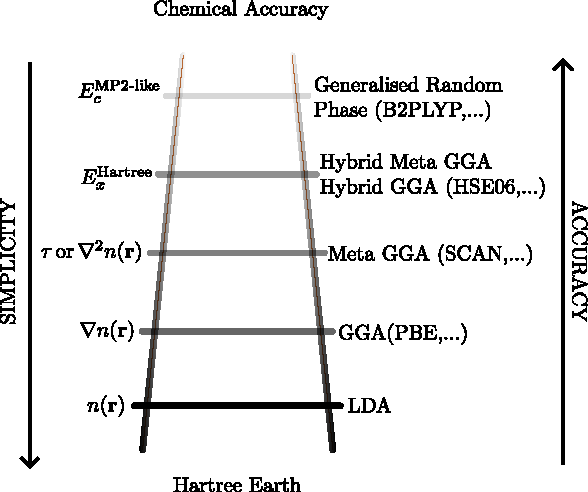
\includegraphics[width=0.6\textwidth]{Jacob-ladder.pdf}
  \caption{Jacob's ladder of exchange-correlation functionals as proposed by J. Perdew\supercite{Perdew2001}. The ladder categorises the functionals into rungs, from the simplest approximation (LDA) at the bottom progressing to more sophisticated and accurate approximations (Generalised Random Phase) at the uppermost rung.  
  }
  \label{fig:jacob-ladder}
\end{figure}

%\section{Density Functional Tight Binding}
%This is a placeholder 

\section{Ab initio Molecular Dynamics} 
Molecular dynamics (MD)\supercite{marx2009ab, Kuhne2014} is a widely used computational method, which allows us to simulate a many-body condensed matter system and to compute its thermodynamic and dynamical properties. In MD, a system is modelled as a collection of particles---atoms or molecules--- whose trajectories evolve over time under the influence of interatomic forces following Newton's equations of motion. 


One of the most challenging, yet crucial, aspects of MD is the calculation of the interatomic forces. In classical MD, these forces are typically computed using predefined potential functions or force fields either constructed upon empirical data or from independent electronic structure calculations that have been parameterised to reproduce experimental or \emph{ab initio} data for small reference systems. Despite their fair success---which we acknowledge but shall not discuss in detail---these empirical interatomic potentials are often limited in their accuracy and transferability. Certain atoms, molecules, or even large systems may give rise to extremely complex interatomic interactions that, if attempted to be modelled with empirical potentials, would demand a rather significant amount of effort. Likewise, these potentials are very often limited to a narrow range of configurations, making them ill-suited for processes involving significant structural changes, such as phase transitions or large deformations.  

Therewith, classical MD can be extended by a first-principles approach, where the interatomic forces are computed on-the-fly from accurate electronic structure calculations, ultimately leading to \emph{ab initio} molecular dynamics (AIMD). This approach allows us to overcome the outlined limitations of classical MD, albeit at a significant computational cost. AIMD employs electronic structure methods such as DFT to compute the interatomic forces at each time step, without relying on predefined interatomic potentials, providing AIMD with an improved predictive power and flexibility.  


\subsection{Hellman-Feynman Theorem}
 The Hellman-Feynman theorem\supercite{Feynman1939, Politzer2018} relates the derivative of the total energy $E$ of a system with respect to a parameter $\lambda$ to the expectation value of the derivative of the hamiltonian with respect to that same parameter. In order to show this, let us consider the following system 

\subsection{Born-Oppenheimer Molecular Dynamics}


\section{Computational Implementation in VASP}
\subsection{Pseudopotentials}
\subsection{K-Point Sampling and Cutoff Energy}
\subsection{Projector Augmented Wave Method}
\subsection{Machine Learning Interatomic Potentials}



